%%
%% This is file `tikzposter-example.tex',
%% generated with the docstrip utility.
%%
%% The original source files were:
%%
%% tikzposter.dtx  (with options: `tikzposter-example.tex')
%% 
%% This is a generated file.
%% 
%% Copyright (C) 2014 by Pascal Richter, Elena Botoeva, Richard Barnard, and Dirk Surmann
%% 
%% This file may be distributed and/or modified under the
%% conditions of the LaTeX Project Public License, either
%% version 2.0 of this license or (at your option) any later
%% version. The latest version of this license is in:
%% 
%% http://www.latex-project.org/lppl.txt
%% 
%% and version 2.0 or later is part of all distributions of
%% LaTeX version 2013/12/01 or later.
%% 








 \documentclass[25pt, a0paper, landscape, margin=0mm, innermargin=15mm,
     blockverticalspace=15mm, colspace=15mm, subcolspace=8mm]{tikzposter} %Default values for poster format options.
% \usepackage{lmodern}
% \makeatletter
% \input{theguy36pt.clo}
% \makeatother
% \usepackage{blindtext}
% \block{Walzing Wombat}{\blindtext}

 \tikzposterlatexaffectionproofon %shows small comment on how the poster was made at bottom of poster

 % Commands
 \newcommand{\bs}{\textbackslash}   % backslash
 \newcommand{\cmd}[1]{{\bf \color{red}#1}}   % highlights command

 % Title, Author, Institute
 \title{LibRoadRunner: High-Performance Timecourse Simulation and Model Fitting}
 \author{J. Kyle Medley, Wilbert Copeland, Kiri Choi, Stanley Gu, Madhav Murthy, Kaylene Stocking and Herbert M. Sauro}
 \institute{University of Washington, Seattle WA}
 \titlegraphic{
\includegraphics[scale=4.0]{SignatureLeftPurple.pdf}}

 % -- PREDEFINED THEMES ---------------------- %
 % Choose LAYOUT:  Default, Basic, Rays, Simple, Envelope, Wave, Board, Autumn, Desert,
 \usetheme{Autumn}
\definecolor{mybannercolor}{rgb}{0.13, 0.055, 0.063}
\definecolor{mybgcolor}{RGB}{232, 229, 206}
\usecolorstyle[colorPalette=BrownBlueOrange,colorTwo=mybgcolor]
{Germany}

\usepackage{pgfplots}
\usepackage{verbatim}
\usepackage{listings}
\usepackage{tabularx}
\usepackage{wrapfig}
\usepackage{amssymb}

\usetikzlibrary{arrows,positioning}

 \begin{document}

     \maketitle

     \begin{columns}%blocks will be placed into columns
         \column{.55}
         \block[roundedcorners=40]{Introduction}{
          {
%             \Large
            Timecourse simulation of kinetic models is an extremely important tool
            in biology, and has found applications in pharmacology (PK/PD models),
            rational design of synthetic systems (Elowitz, \textit{Nature} 2000),
            and whole-cell model simulation (Karr, \textit{Cell} 2012).
            Pushing the envelope of high-speed model simulation is key to exploring
            more complex and diverse biological modeling approaches.

            \textbf{libRoadRunner} is designed to be a high-performance simulator and analysis
            library for SBML-encoded models.
            To facilitate maximum performance, libRoadRunner makes use of the LLVM library
            (\texttt{llvm.org}) to compile models to native machine code which can be
            executed directly on the target CPU.

            By using an open and transparent development process, making our source code
            freely available, and working extensively with our collaborators through
            weeklong workshops, we have enabled widespread access to this powerful
            modeling tool.
          }

          \vspace{50pt}

          \begin{tikzfigure}[The libRoadRunner native compilation pipeline]
            \begin{tikzpicture}[->,>=stealth',very thick]
              \node (sbmllogo) {
\includegraphics[scale=6.0]{sbml-logo.pdf}};
              \node (ircode)[right= 3 of sbmllogo, align=left] {
              \small\texttt{define internal double}\\
              \small\texttt{@getFloatingSpeciesConcentration}\\
              \small\texttt{(\%rr\_LLVMModelData* \%modelData, i32 }\\
              \small\texttt{entry: switch i32 \%floatingSpeciesIndex}
              };
              \node (machinecode)[right= 3 of ircode, align=left] {
              \small\texttt{  7c2b20:  55                    push   \%rbp}\\
              \small\texttt{  7c2b21: 48 89 e5              mov    \%rsp,\%rbp}\\
              \small\texttt{  7c2b2e: 5d                    pop    \%rbp}\\
              \small\texttt{  7c2b2f: c3                    retq}
              };
              \node (simplot)[right= 3 of machinecode] {
                \begin{tikzpicture}
                  \begin{axis}[
                    width=0.10\textwidth,
                    height=0.09\textheight,
                    xlabel=$t$,
                    domain=0:1,
                    xtick=\empty,%{0,0.25,0.75,1},
                    ytick=\empty,
                    axis lines = middle,
                    enlargelimits = true,
                    axis line style = very thick] %http://tex.stackexchange.com/questions/237709/pgfplots-ignores-thick-option-for-axes
                    \addplot[smooth,mark=*,blue] {x^2*(1+sin(deg((x*5)^2)))};
                    \addlegendentry{$f(t,p)$}
                  \end{axis}
                \end{tikzpicture}
              };

              \path
                (sbmllogo) edge[line width=5pt] node [left] {} (ircode)
                (ircode) edge [right,line width=5pt] node[left] {} (machinecode)
                (machinecode) edge [right,line width=5pt] node[left] {} (simplot) ;

              \node [below= of sbmllogo] {\textbf{SBML Model}} ;
              \node [below= of ircode] {\textbf{LLVM IR Code}} ;
              \node [below= of machinecode] {\textbf{Native Machine Code}} ;
              \node [below= of simplot] {\textbf{Simulation}} ;
            \end{tikzpicture}
          \end{tikzfigure}

          \vspace{50pt}

          \innerblock[]{Native Performance}{libRoadRunner uses a non-tracing JIT to run simulations with the speed of a native executable}
%             \coloredbox{Text may be highlighted using colored boxes created by \bs\texttt{coloredbox[{\it options}]\{{\it Text\}}}}

          \vspace{1.5em}

     }
     \block{Model Fitting}{
         libRoadRunner's performance allows for the use of expensive fitting and optimization algorithms.
         We used libRoadRunner to optimize a dye-binding model for quantifying promoter activity
         using \textbf{differential evolution}, a heuristic optimization method.

          \begin{tikzfigure}[Malachite green aptamer model and plot courtesy of Wilbert Copeland]
            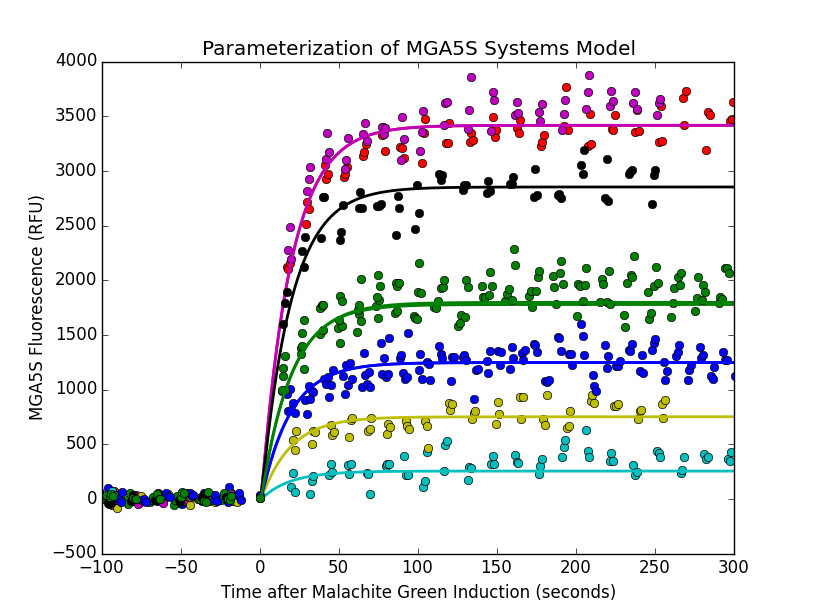
\includegraphics[scale=0.8]{figure1.png}
            \hspace{8em}
            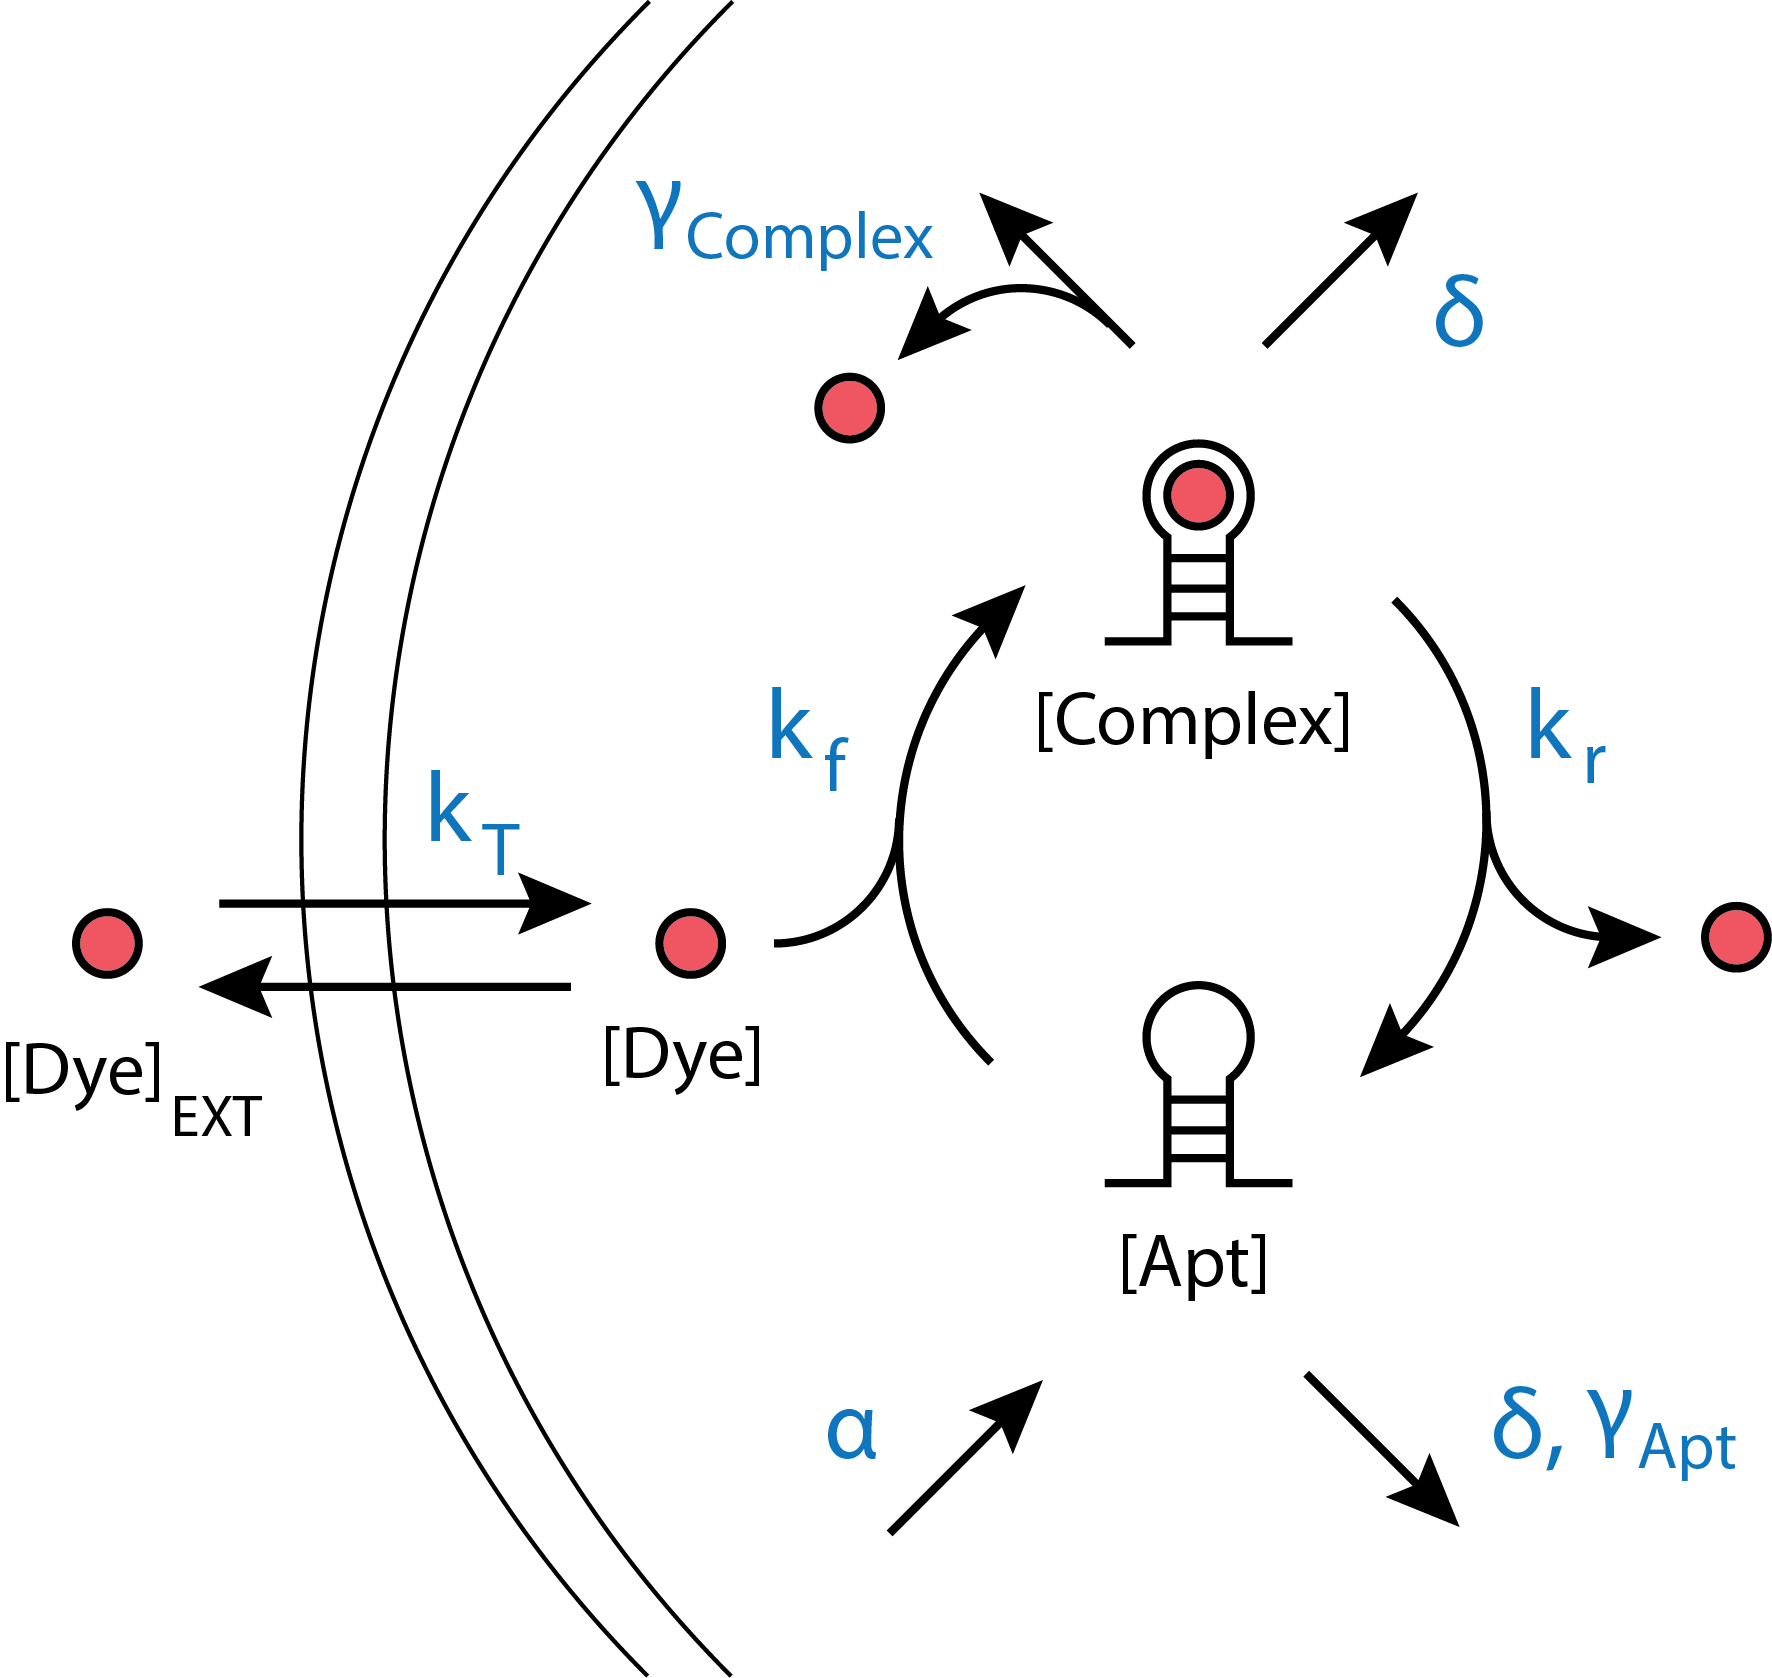
\includegraphics[scale=0.8]{SystemDiagramWC083115.png}
          \end{tikzfigure}
     }

%      \note[targetoffsetx=24cm, targetoffsety=-9cm,rotate=1,angle=270,radius=8cm,width=.75\textwidth,innersep=.4cm]{
%          You can place notes that are ``attached'' to the previous block using the command
%          \begin{quote} \texttt{\bs note[{\it options}]\{{\it contents}\}}\end{quote}
%          The note is placed by default slightly to the right of a ``target'' in the center of the previous block.  The note style may also allow for a connection between the note and the ``target''.  \\
%          The target may be shifted from the default by setting the options  \texttt{targetoffsetx, targetoffsety}, rotated by an angle with \texttt{rotate}, and its width with \texttt{width}.  The placement of the note in relation with the target is given in polar coordinates with \texttt{ radius, angle}. Please observe that notes are always drawn {\bf over} the other objects. They do not affect the placement of blocks.
%       }
     \note[targetoffsetx=18cm,targetoffsety=-3cm,innersep=.4cm,angle=-45,connection]{A model predicts aptamer state based on kinetic parameters}
     \note[targetoffsetx=-4cm,targetoffsety=-1.5cm,innersep=.4cm,angle=45,connection]{Parameters can be fitted from fluorescence data}

    \column{.45}
      \block{Under the Hood}{
          Our C++ library features a modular design, allowing effortless upgrades to its internal architecture.
          The library features pure, abstract base classes for \textbf{integrators} and \textbf{steady-state solvers}.
          Using these interfaces, we have implemented a timecourse integrator (\textit{CVODE}) from the
          Lawrence Livermore National Laboratory's \textit{SUNDIALS} suite.
          CVODE features an Adams-Moulton method for non-stiff problems, and a Backwards Differentiation
          Formula (BDF) in fixed-leading coefficient form for stiff problems. %https://computation.llnl.gov/casc/sundials/description/description.html
          For locating steady states, libRoadRunner uses the NLEQ library (Nowak and Weimann, 1991),
          a damped Newton method for highly nonlinear equations.
          \innerblock[]{APIs}{libRoadRunner features APIs for C, Python, and Java, enabling it to be used from any of these languages}
      }
%          \block{Columns}{
%               By default, blocks are arranged in a single column. If you want multiple columns for your poster, you may use the \texttt{columns} environment. For example,
%              \begin{quote}
%                  \texttt{\noindent \bs begin\{columns\}\\
%                  \bs column\{.6\}\\
%                  \bs block\{\dots\}\{\dots\}\\
%                  \bs column\{.4\}\\
%                  \bs block\{\dots\}\{\dots\}\\
%                  \bs block\{\dots\}\{\dots\}\\
%                  \bs end\{columns\}
%                  }
%              \end{quote}
%              will create two columns of 60\% and 40\% the available width; spacing between successive columns is handled automatically.  The block command(s) following \texttt{\bs column} are the blocks to go in that column.  The number of columns is free to be chosen, but the relative widths must all be chosen.  If the widths sum to less than 1, empty space will be seen on the right.  If they sum to more than 1, the latter columns will be cut off.
%          }

         \begin{subcolumns}
            \subcolumn{.45}
            \block{Platform Support}
            {By utilizing the diverse code generation targets included with LLVM,
            we can deploy libRoadRunner on a variety of platforms, including embedded
            RISC architectures such as ARM.

%             \vspace{2.5em}

%             Utilizing a group of three networked NVidia TK-1 devices (right),
%             we implemented an asynchronous, distributed computing engine based on
%             the $\varnothing$MQ library. This capability is used to run simulation
%             jobs in the
            We have created a simulation queue service which recruits computing nodes to run extremely large numbers of simulations, which may drastically reduce the run-time necessary for certain types of analysis, such as Monte Carlo or evolutionary algorithms.
            }

            \subcolumn{.5}
            \block{}{
              \begin{tikzfigure}[NVidia Jetson TK-1 (top) and Adapteva Parallella (bottom)]
                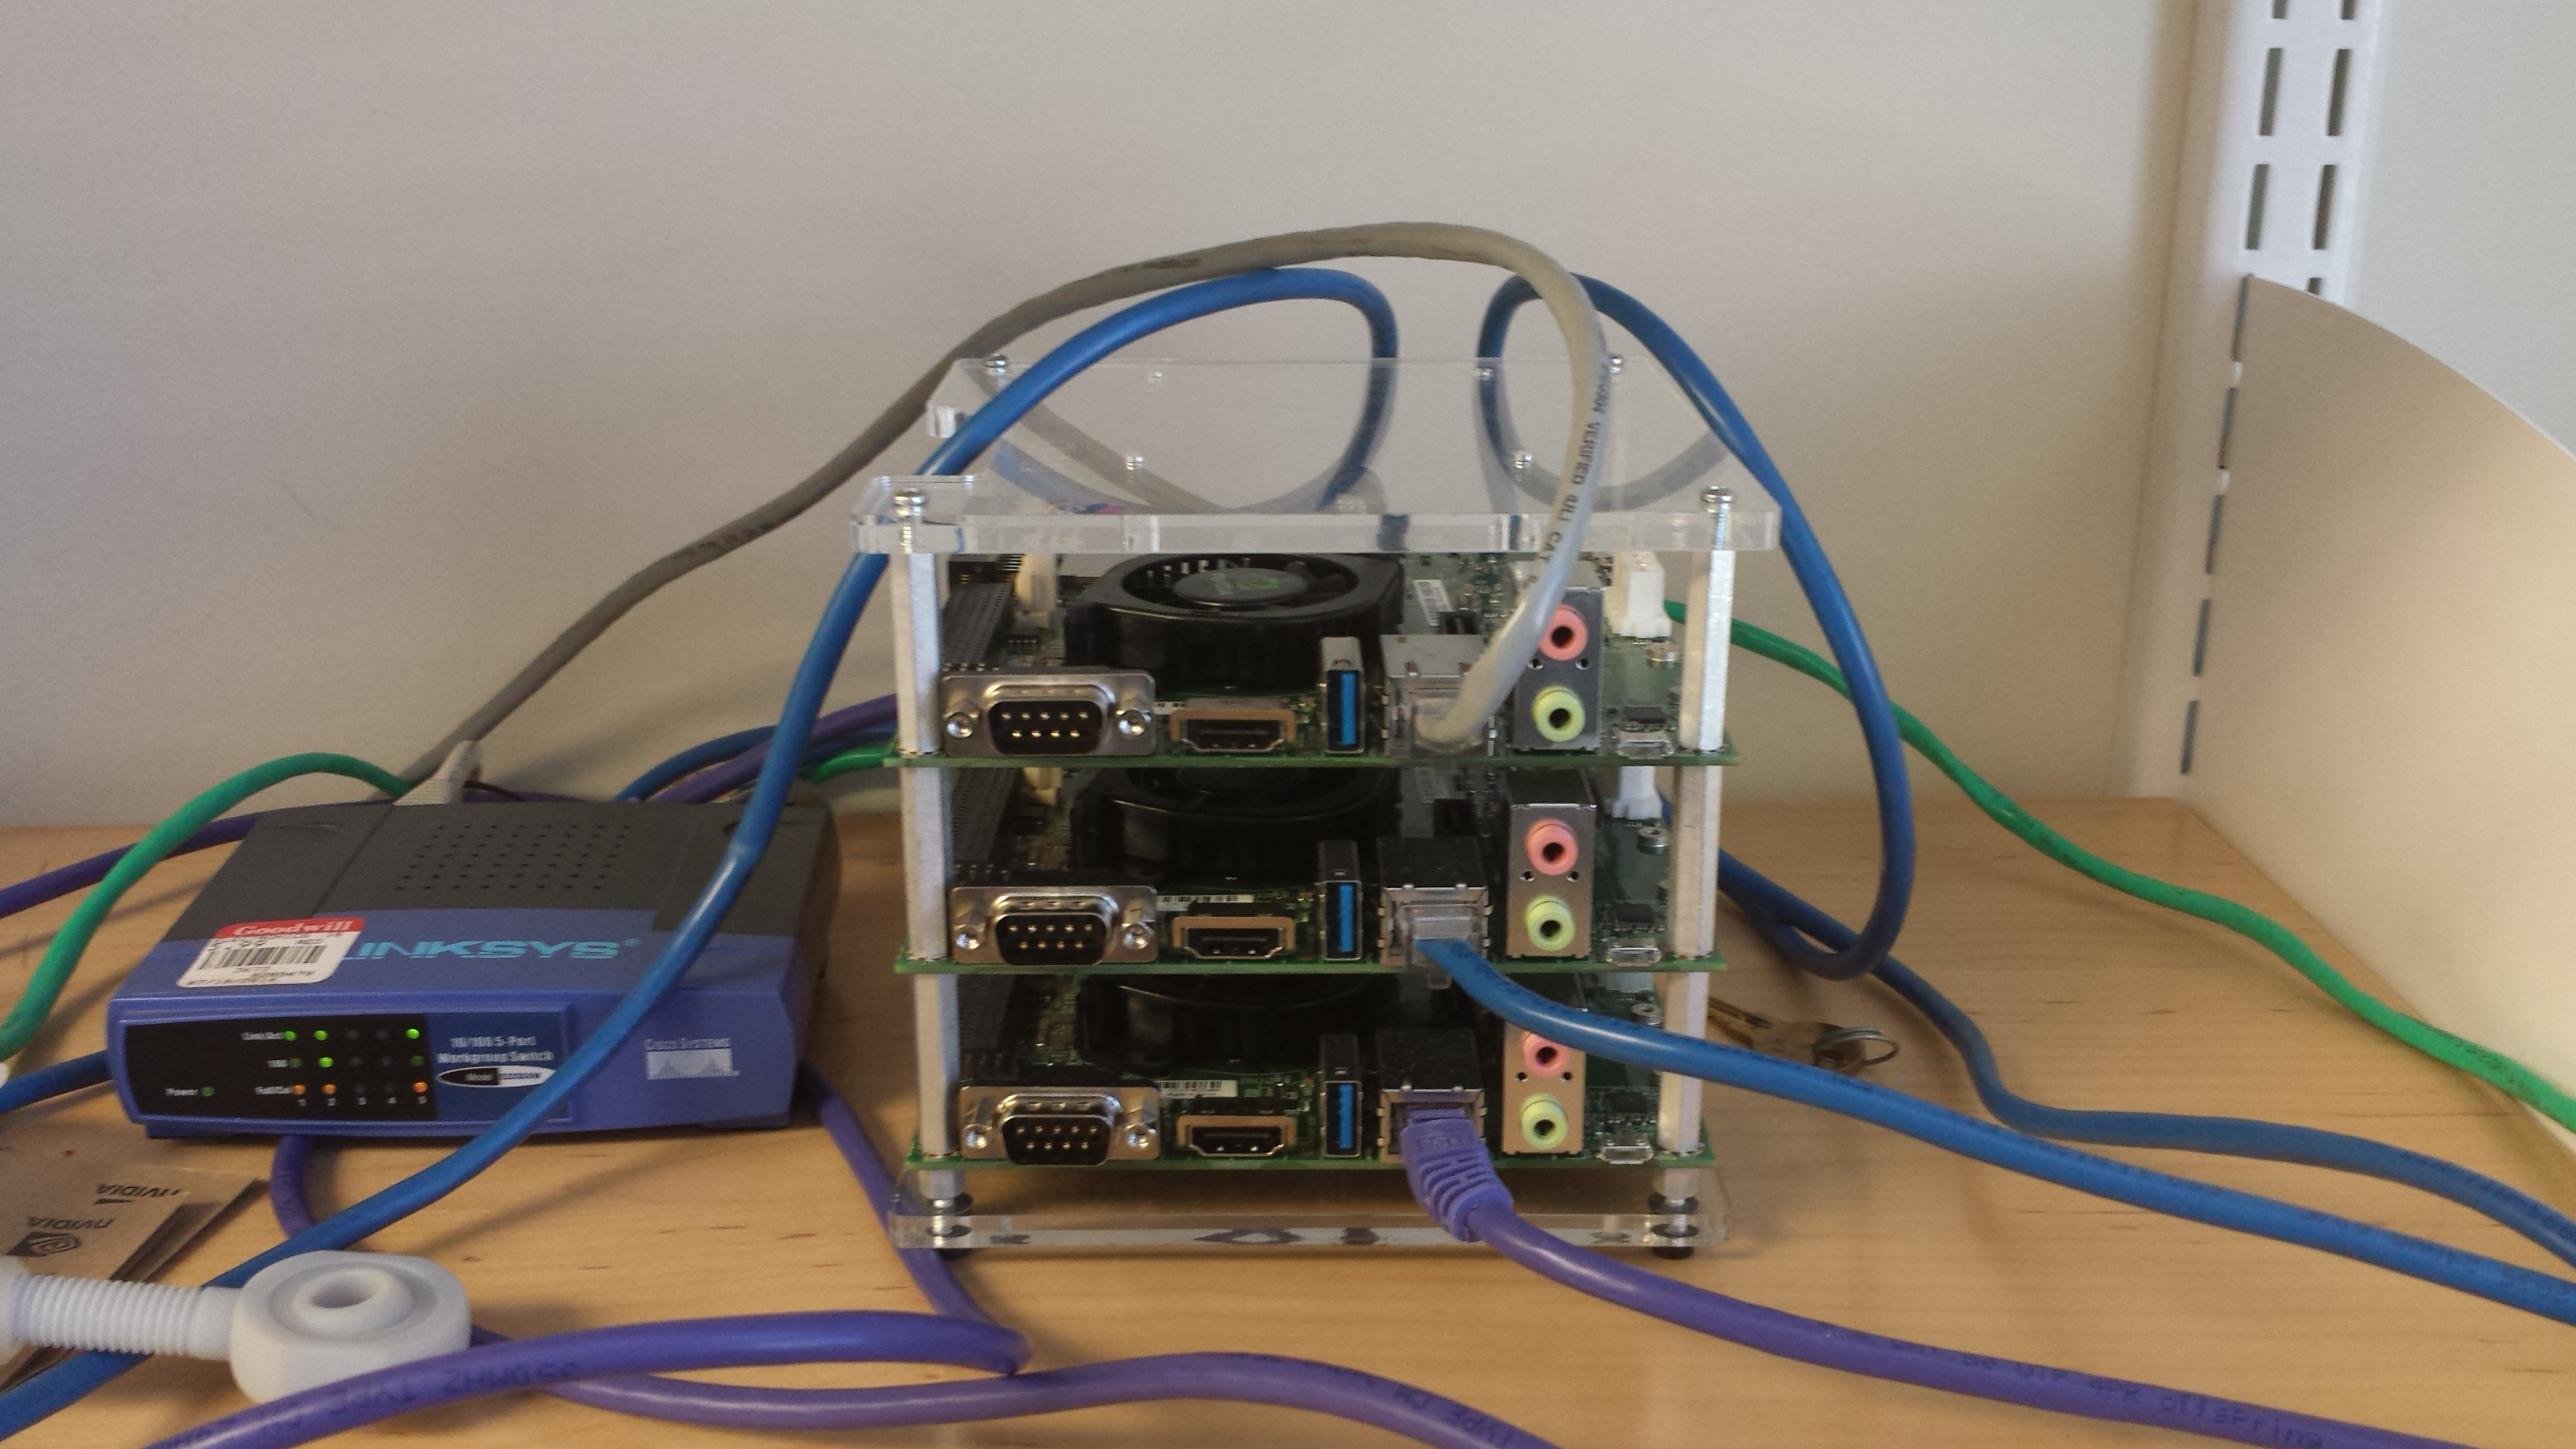
\includegraphics[scale=0.10]{tk1cluster.jpg}
                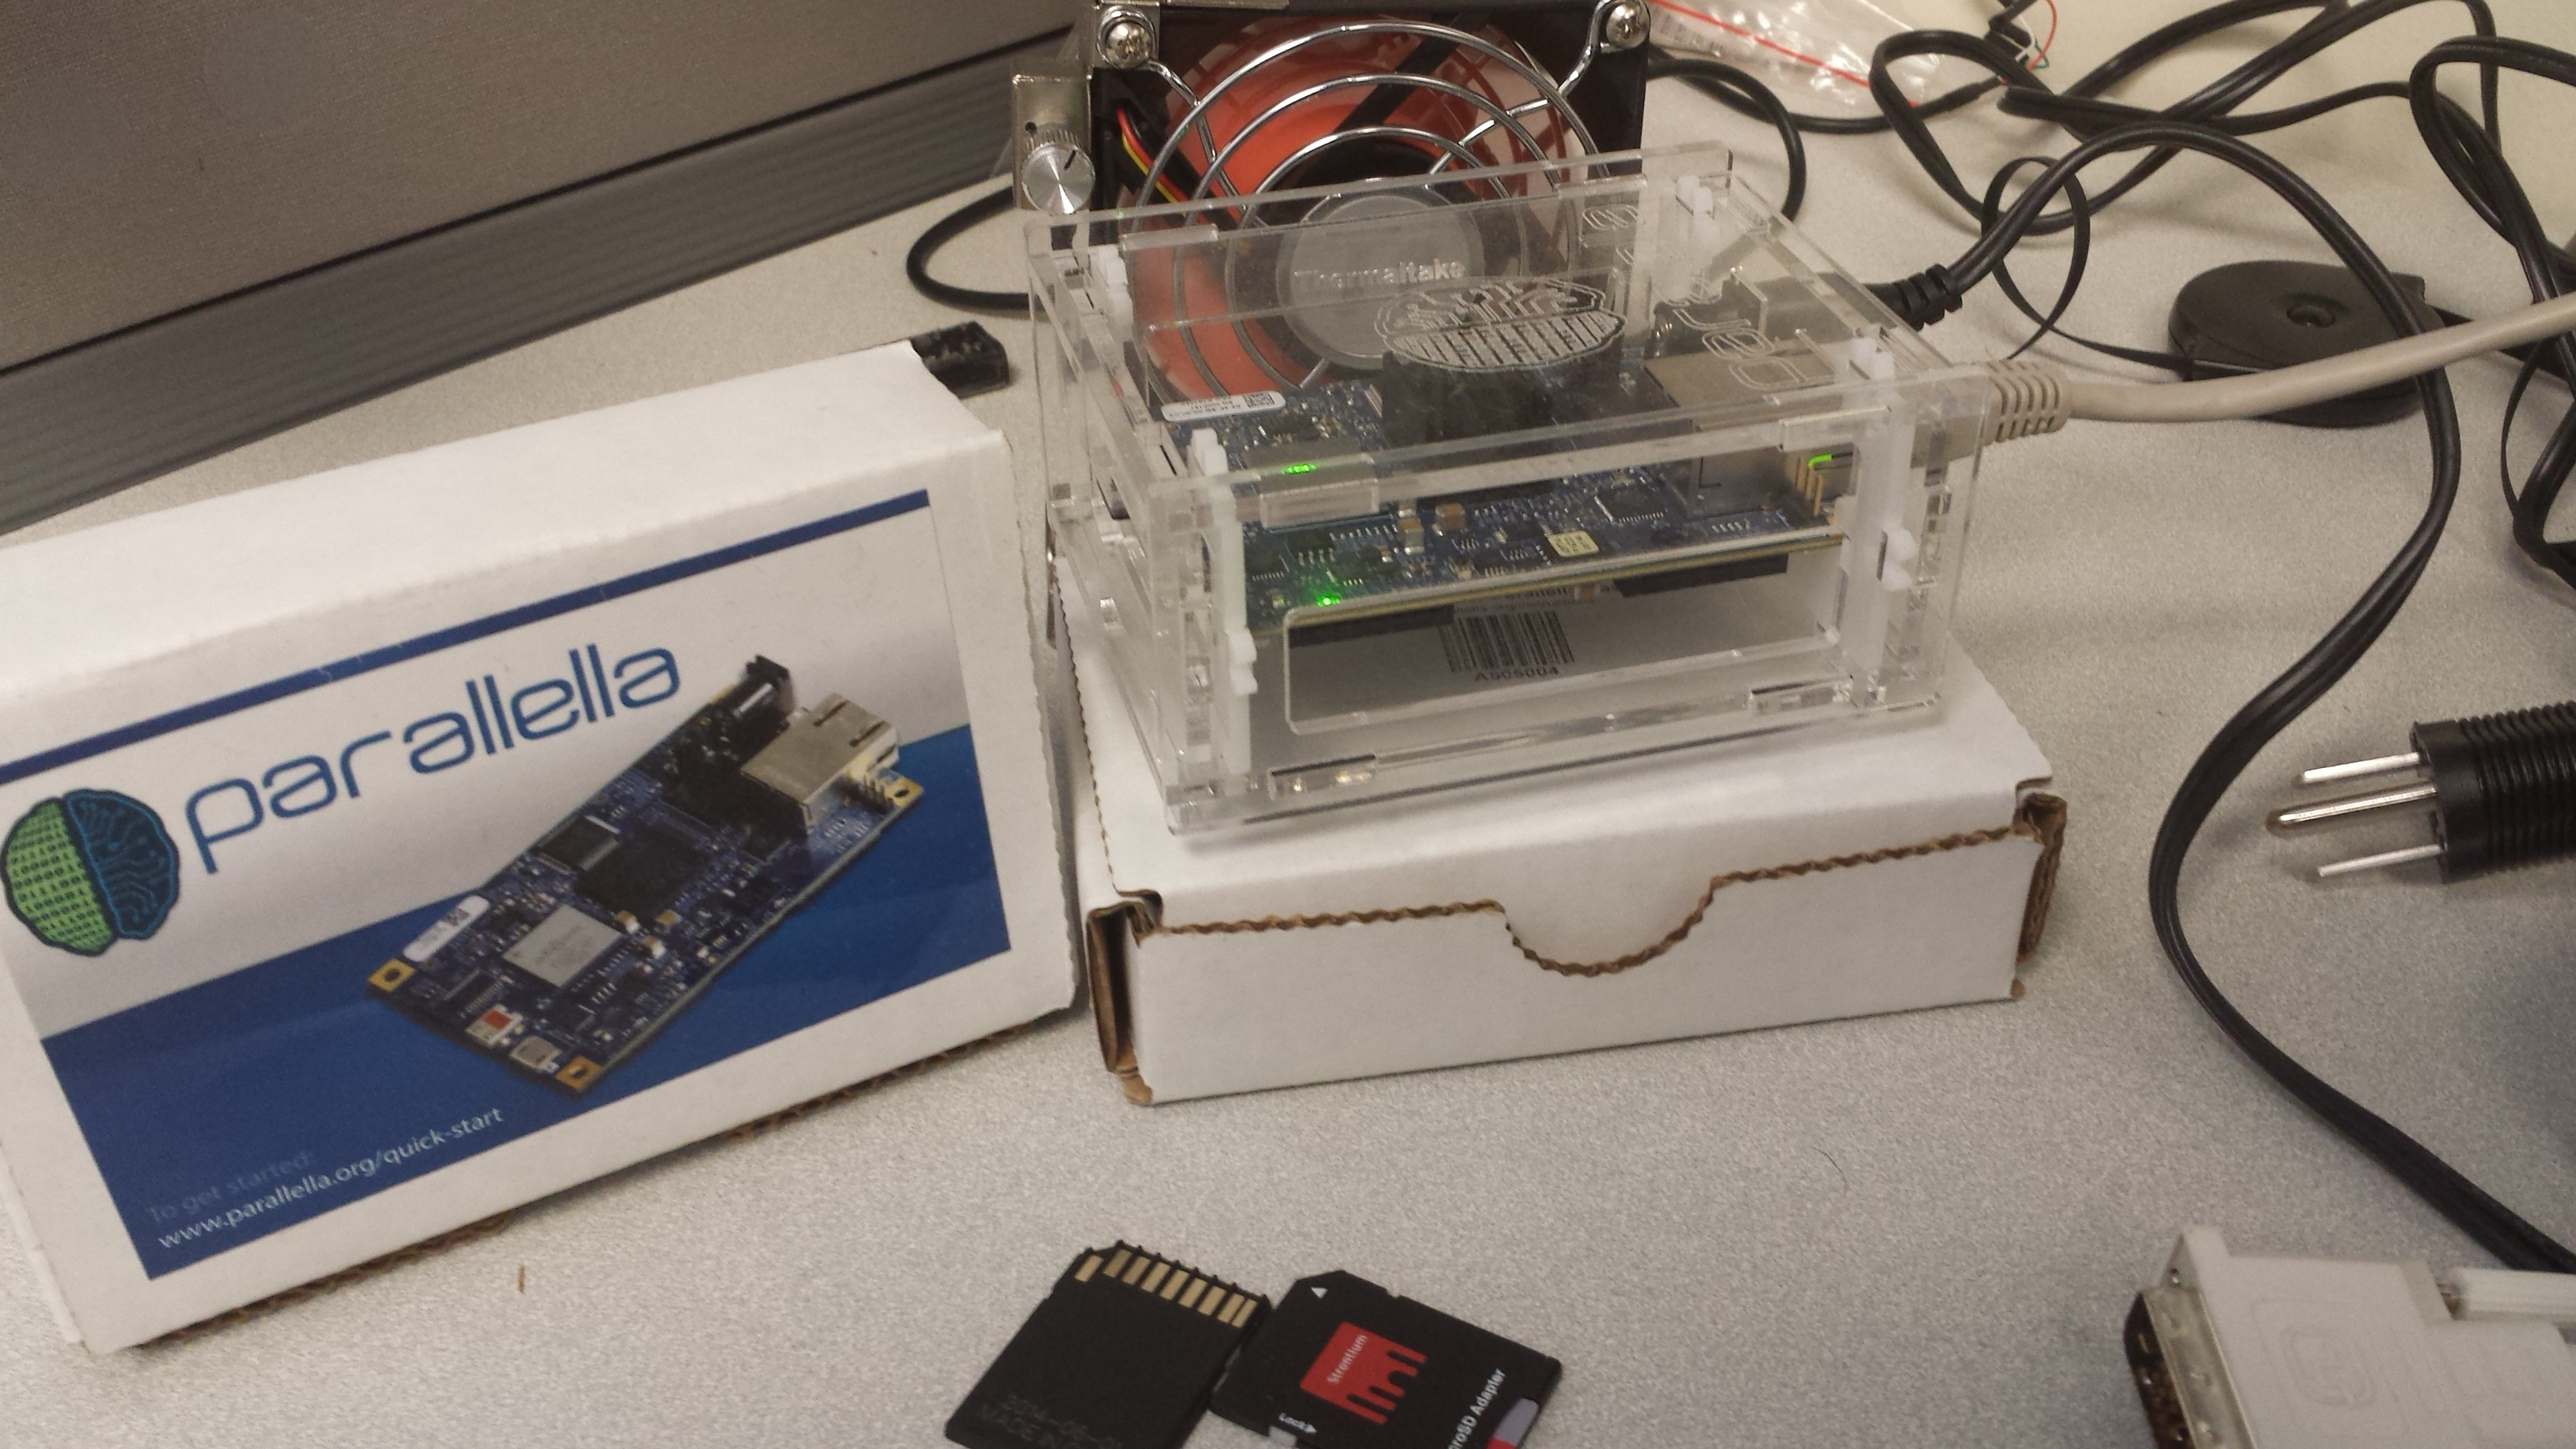
\includegraphics[scale=0.10]{parallella.jpg}
              \end{tikzfigure}
            }
         \end{subcolumns}

%          \block[titlewidthscale=.8,bodywidthscale=.9,titleoffsety=9.5mm,bodyoffsety=9mm]{Changing the Poster's Appearance}{
          \block{Acknowledgments and Funding Sources}{
            \begin{tikzfigure}
            \centering
            
\includegraphics[scale=0.32]{nigms.png}
            \hspace{8em}
            
\includegraphics[scale=0.9]{DeptBioEnguw.pdf}
            \end{tikzfigure}

            We wish to acknowledge Andy Somogyi for his extensive work on libRoadRunner
            (in particular, for writing the LLVM simulation engine).
            We also acknowledge Totte Karlsson for the original C\# to C++ translation, C compiler backend and C API, Lucian Smith for developing part of the test suite, and Michael Galdzicki for writing detailed build instructions and testing for developers.
            We are deeply indebted to the feedback from our collaborators
            Jean-Marie Bouteiller at the University of Southern California,
            Maciej H. Swat and James A. Glazier at the Biocomplexity Institute, Indiana University, and
            Matthias K\"{o}nig at Charit\'{e} --- Universit\"{a}tsmedizin Berlin.
            This work was funded by generous support from NIH grant R01 GM081070. The content is solely the responsibility of the authors and does not necessarily represent the views of the National Institutes of Health.

%             \vspace{1em}

            Logos are copyright their respective owners.

%             \vspace{1em}

%             \begin{tikzfigure}
%             \centering
%             
\includegraphics[scale=1.0]{DeptBioEnguw.pdf}
%             \end{tikzfigure}
          }

     \end{columns}

     \block[]{}{
%      \block[titleoffsety=-1cm,bodyoffsety=-1cm]{Sample document}{
      \resizebox{0.95\textwidth}{!}{ %http://tex.stackexchange.com/questions/121155/how-to-adjust-a-table-to-fit-on-page
        
\includegraphics[scale=0.35]{libroadrunner_logo_tan.jpg}
        \hspace{20em}
        
\includegraphics[scale=5.0]{sbml-logo.pdf}
        \hspace{20em}
        
\includegraphics[scale=0.8]{SEDMLlogo.png}
        \hspace{20em}
        
\includegraphics[scale=0.17]{LLVMLogoTight.pdf}
        \hspace{20em}
        
\includegraphics[scale=0.6]{TelluriumLogo.png}
        \hspace{20em}
        
\includegraphics[scale=0.5]{python-powered-w.pdf}
        \hspace{20em}
        
\includegraphics[scale=3.5]{inventing-the-future-of-medicine-outlines.pdf}
      }
%      \vspace{2em}
%          This poster was created by the following commands (omitting the contents of the blocks and notes) to give a sense of how different objects are created and options used.
%          \begin{quote}
%              \texttt{\bs documentclass[25pt, a0paper, landscape, margin=0mm, innermargin=15mm,
%          blockverticalspace=15mm, colspace=15mm, subcolspace=8mm]\{tikzposter\}\\
%              \bs title\{Using tikzposter\} \bs author\{Pascal Richter, Elena Botoeva, Richard Barnard, \& Dirk Surmann\} \bs institute\{\}\\
%               \bs usetheme\{Autumn\}\bs usecolorstyle[colorPalette=BrownBlueOrange]\{Germany\}\\
%              \bs begin\{document\}\bs maketitle\\
%              \bs begin\{columns\} \bs column\{0.55\}\\
%              \bs block\{Creating the document\}\{The document\dots\} \bs note[targetoffsetx=-.05\bs textwidth,targetoffsety=9.5cm,innersep=.4cm,angle=-45,connection]\{\dots\}\\
%              \bs block\{The title matter\}\{The title\dots\}\\
%              \bs block\{Blocks\}\{Blocks are\dots\} \bs note[targetoffsetx=24cm, targetoffsety=-9cm,rotate=1,angle=270,radius=8cm,width=.75\bs textwidth,innersep=.4cm]\{You can\dots\}\\
%              \bs column\{0.45\} \bs block\{Columns\}\{By default,\dots\}\\
%              \bs begin\{subcolumns\} \bs subcolumn\{.45\}
%              \bs block\{Subcolumns\}\{If you\dots\}
%              \bs subcolumn\{.5\} \bs block\{\}\{An example\dots\}
%              \bs end\{subcolumns\}\\
%              \bs block[titlewidthscale=.8,bodywidthscale=.9,titleoffsety=9.5mm,bodyoffsety=9mm]\{Changing the Poster's Appearance\}\{If the default\dots\}
%              \bs end\{columns\}\\
%              \bs block[titleoffsety=-1cm,bodyoffsety=-1cm]\{Sample document\}\{This poster\dots\}\\
%              \bs end\{document\}
%              }
%          \end{quote}
     }

 \end{document}




\endinput
%%
%% End of file `tikzposter-example.tex'.
